\documentclass[a4paper,article,14pt]{extarticle}

% Подключаем главный пакет со всем необходимым
\usepackage{items/spbudiploma}

% Пакеты по желанию (самые распространенные)
% Хитрые мат. символы
\usepackage{euscript}
% Таблицы
\usepackage{longtable}
\usepackage{makecell}
% Картинки (можно вставлять даже pdf)
\usepackage[pdftex]{graphicx}

\usepackage{amsthm,amssymb, amsmath}
\usepackage{textcomp}

% \usepackage{minted} % для примеров кода (требует параметра -shell-escape)
% \usemintedstyle{bw}
\usepackage{float}
% \subcaptionbox для нескольких картинок в ряд
\usepackage{subcaption}

\begin{document}

% Титульник в файле titlepage.tex
\newgeometry{left=30mm, top=20mm, right=15mm, bottom=20mm, nohead, nofoot}
\begin{titlepage}
\begin{center}

\textbf{Санкт--Петербургский государственный университет}\\
\textbf{Факультет математики и компьютерных наук}


\vspace{35mm}

\textbf{\textit{\large Можаев Андрей Михайлович}} \\[8mm]
% Название
\textbf{\large Выпускная квалификационная работа}\\[3mm]
\textbf{\textit{\large Разработка метода построения упрощенной динамической модели для задачи оптимального управления микроклиматом помещения}}

\vspace{20mm}
Уровень образования: бакалавриат\\
Направление 01.03.02 «Прикладная математика и информатика»\\
Основная образовательная программа СВ.5156.2019
«Прикладная математика, фундаментальная информатика и программирование»\\
Профиль «Современное программирование»\\[25mm]


% Научный руководитель, рецензент
\begin{flushright}
\begin{minipage}[t]{0.65\textwidth}
{Научный руководитель:} \\
к.ф.-м.н. Дмитрий Сергеевич Шалымов
\vspace{10mm}

{Рецензент:} \\
зав. лаб. 37 в ИПУ РАН,\\
д.т.н Антон Викторович Уткин, 
\end{minipage}
\end{flushright}

\vfill

{Санкт-Петербург}
\par{\the\year{} г.}
\end{center}
\end{titlepage}
\restoregeometry
\addtocounter{page}{1}


% Содержание
\tableofcontents
\pagebreak

\specialsection{Введение}

Данное исследование является частью проекта по созданию централизованной системы управления потреблением энергии в зданиях общего назначения, тепловой и электрической. Одной из уникальных особенностей данной системы предполагается разработка и последующее применение интеллектуальных методов предсказания энергопотребления. Для предсказания энергопотребления надо понимать и уметь измерять те факторы, которые определяют необходимое количество электричества и тепла для здания в этот момент и в ближайшие несколько часов.

При постановке задачи регулирования для систем отопления, кондиционирования и вентиляции (ОВК), эксплуатирующие службы руководствуются двумя конкурирующими критериями: экономичностью работы системы и комфортностью внутренней среды. По различным оценкам, от 50 до 70 процентов всей расходуемой энергии приходится на ОВК. Таким образом, оптимизация потребления этого класса устройств, пусть даже на 5-10 процентов, повлечет за собой ощутимое снижение общего уровня расхода энергии. 

В основе данной работы лежит идея скомбинировать два основных подхода к моделированию микроклимата помещений: методы вычислительной термодинамики \cite{cfd}(CFD) и методы сетевых воздушных потоков (NAF). Точное решение задачи CFD на небольшом временном промежутке позволит смоделировать работу измерительного комплекса, оптимизировать вектор измеряемых величин, количество датчиков и их расположение в помещении. 


\newpage

\specialsection{Постановка задачи}

Основной вопрос - где в помещении расположить датчик температуры, который будет использоваться в составе централизованной системы эксплуатации здания, направленной на оптимизацию энергопотребления и обеспечение комфорта внутренней среды? Подобные системы используют методы управления с предсказывающими моделями. Поэтому предлагается критерий размещения датчика, учитывающий качество регресионных моделей, получаемых на основе показаний. 

Эта задача решается численными методами, так как сбор данных эмпирическим путем займет много времени и ресурсов. В стандартных офисных зданиях число отдельных зон может доходить до нескольких сотен, поэтому расстановка датчиков и считывание показаний очень трудоемкий процесс. В то же время, используя сгенерированную модель, мы можем определить значения на датчиках одновременно для всех интересующих расположений.

Для сокращения времени обследования здания, ускорения процесса развертывания сети, было предложено выделить в проекте два этапа - численное моделирование исследуемого помещения и анализ полученных данных.

На первом этапе будет смоделирован "Демонстрационный стенд Умного дома". Геометрия помещения задана в формате CAD. Моделирование будет производится в COMSOL Multyphysics \cite{comsol}. Целью является моделирование некоторого промежутка времени с хорошей точностью. Будет смоделирован процесс теплообмена внутри помещения и с окружающим воздухом, а также солнечная радиация. Значения внешней температуры будут взяты из собранного ранее датасета. Полученная модель будет использована далее.

На втором этапе будут выбраны точки возможного расположения датчика. Температуры в них будут импортированы в таблицу. Дальнейшая работа с полученными таблицами будет реализована на языке Python. Проанализировав потенциальные места расположения датчика методом, который предлагают в своей статье Пащенко А.Ф., Рассадин Ю.М. \cite{pashchenko-rassadin} (подробней об этом методе в главе \ref{algo-2}), сравнительным анализом найдем наилучшую точку размещения микроклиматического датчика. Для небольших помещений достаточно перебора потенциальных точек размещения, для больших помещений со сложной конфигурацией возможно применение градиентного метода поиска.


Результатом дипломного проекта станет отработанный метод построения упрощенной динамической модели характеристик воздуха в помещении, на основе которой может быть реализован последующий сбор реальных данных.

\newpage

\specialsection{Обзор предметной области}

Существуют два основных подхода моделирования микроклимата помещения \cite{ashrae}: метод вычислительной гидродинамики (CFD) и метод сетевых воздушных потоков (NAF). У каждого из этих подходов свои преимущества и недостатки.

Метод вычислительной гидродинамики может быть использован для моделирования помещения с микроскопической точностью. Динамика состояния помещения моделируется системой дифференциальных уравнений Навье-Стокса. Задаются геометрия помещения и граничные условия. В общем случае граничное условие определяет физическую задачу в определенных положениях. Часто физические явления осложняются одновременными тепловыми потоками (например, теплопроводностью через ограждение здания, получением тепла от обогреваемых внутренних объектов, солнечным излучением через остекление здания), фазовыми изменения (например, конденсация и испарение воды), химические реакции (например, горение) и механические перемещения (например, вентиляторы, перемещения жильцов).

Первым шагом в проведении CFD-анализа является разделение области на большое количество более мелких областей, называемых ячейками. Совокупность ячеек, составляющих область интереса, обычно называется сеткой или решеткой. Размер ячеек позволяет контролировать точность расчета.

CFD включает в себя решение связанных дифференциальных уравнений в частных производных, которые должны решаться одновременно или последовательно. Аналитических решений для моделирования внутренней среды не существует. Компьютерные численные процедуры являются единственным средством получения полных решений этих наборов уравнений.

Однако, высокая точность CFD компенсируется большими временными затратами как для аналитика при построении модели и интерпретации результатов, так и при решении компьютером смоделированных уравнений. Это ограничивает использование CFD для достаточно простых помещений и стационарных решений.

Существует достаточно много инструментов для моделирования, среди них: COMSOL Multyphysics \cite{comsol}, SimScale \cite{simscale}, EnergyPlus \cite{energyplus}, TRNSYS \cite{trnsys}

\newpage

В свою очередь, метод сетевых воздушных потоков может дать макроскопическое представление о здании путем решения системы уравнений сохранения массы и энергии. Сетевые модели воздушного потока идеализируют здание как совокупность зон, таких как комнаты, коридоры и места соединения воздуховодов, соединенных путями потока, представляющими двери, окна, вентиляторы, воздуховоды и т.д. Таким образом, пользователь собирает описание здания, соединяя зоны с помощью соответствующих путей потока. Сетевая модель прогнозирует потоки воздуха от зоны к зоне на основе характеристик давления и расхода в моделях путей и различий в давлении на путях. Три типа сил управляют потоком по путям: ветер, перепады температур (эффект стекания) и механические устройства, такие как вентилятор.

Как показано на рис. \ref{NAF}, модели сетей воздушного потока напоминают электрические сети. Поток воздуха соответствует электрическому току, при этом давление в зоне действует подобно напряжению в электрическом узле. Пути прохождения потока реагируют на резисторы и другие электрические элементы, включая активные элементы, такие как батареи (вентиляторы).

Весь этот процесс занимает гораздо меньше времени, что делает возможным моделирование всего здания, включая различные механические системы, в течение периода времени продолжительностью до года. Ограничения этого метода включают в себя гораздо менее детализированные результаты (например, отсутствие сведений о потоке воздуха внутри помещения). Отсутствие детализации в моделях зон сети делает CFD предпочтительным для прогнозирования теплового комфорта или проектирования систем вытесняющей вентиляции, где структура воздушного потока в помещении определяет интересующие величины.

Идея совместить эти два подхода была описана ранее в статье "Оптимизация HVAC-систем с помощью моделирования" \cite{blog}. Было смоделировано офисное помещение и находилось расположение датчика, который использовался для определения, в какой момент включать кондиционер. Тем не менее, авторы не ставили перед собой задачу придумать алгоритм, который позволит это делать для произвольной модели.

\begin{figure}[H]
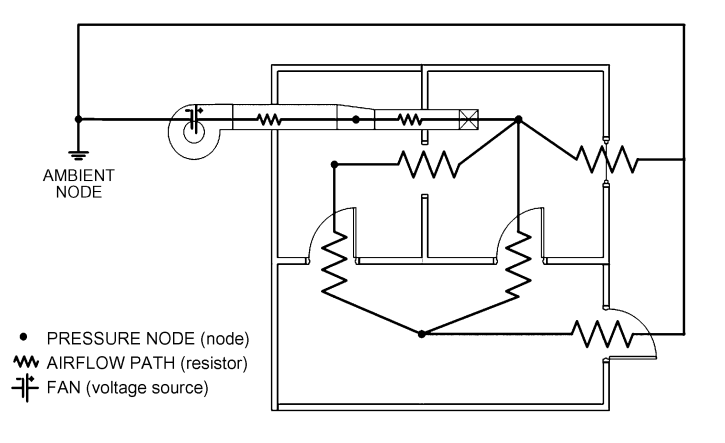
\includegraphics[width=\textwidth]{images/NAF_example.png}
\caption{}
\label{NAF}
\end{figure}



\graphicspath{{./images/model}}
\section{Построение модели}

Целью данного этапа является построение модели <<демонстрационного стенда Умного дома>>, которая затем будет использована для определения оптимального расположения датчика температуры. В качестве платформы для моделирования был выбран COMSOL Multiphysics.


\subsection{Построение модели куба}

В начале работы было решено создать простую модель деревянного куба с ребром $1$ метр и толщиной стен $15$ сантиметров, а затем проанализировать изменение температуры внутри. Для создания физической модели использовался SolidWorks, а затем модель была импортирована в COMSOL. В COMSOL внутренность куба заполнили воздухом (куб воздуха с ребром $0.7$ м), материал стен выбран как Wood (pine).

Начальная температура стен и воздуха внутри $293$ К. Температура, действующая на внешнюю поверхность стен куба, задана по формуле:
\[300 + 50 \cdot \sin(\frac{\pi \cdot t[s]}{500}) K\]

Промоделлирован промежуток времени длиной $1000$ секунд с шагом $50$.
Были рассмотрены различные размеры сетки разбиения: Normal (Рис. \ref{cube-normal}), Fine (Рис. \ref{cube-fine}), Finer (Рис. \ref{cube-finer}) и Extra fine (Рис. \ref{cube-extra-fine}).

Ниже можно увидеть полученные результаты. На первой картинке изображена сама сетка, на второй и третьей температура в разрезе в момент 250 и 750 секунд соответственно.

\begin{figure}[H]
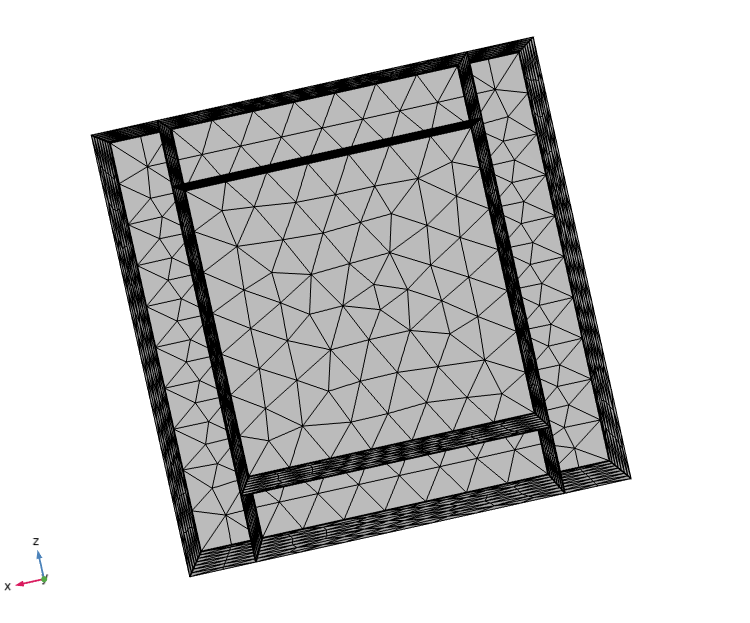
\includegraphics[width=0.3\textwidth]{cube/normal_mesh.png}\hfill
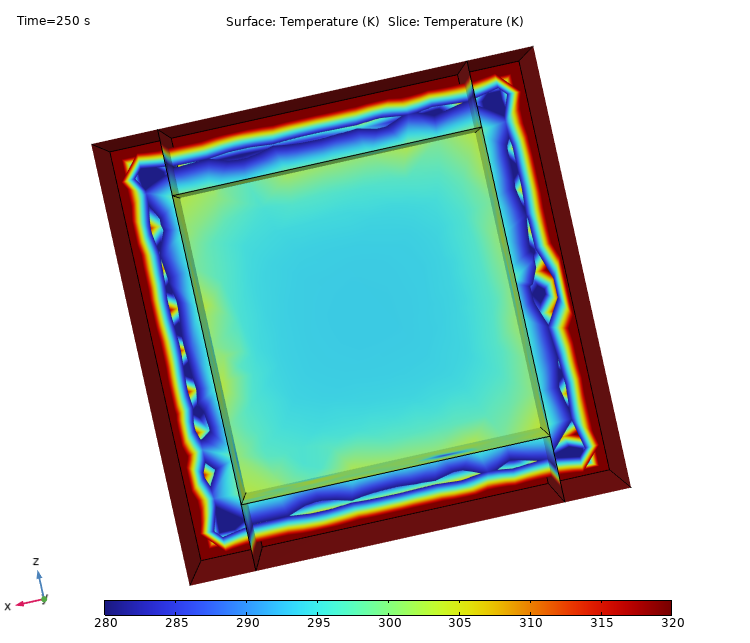
\includegraphics[width=0.3\textwidth]{cube/normal_250s.png}\hfill
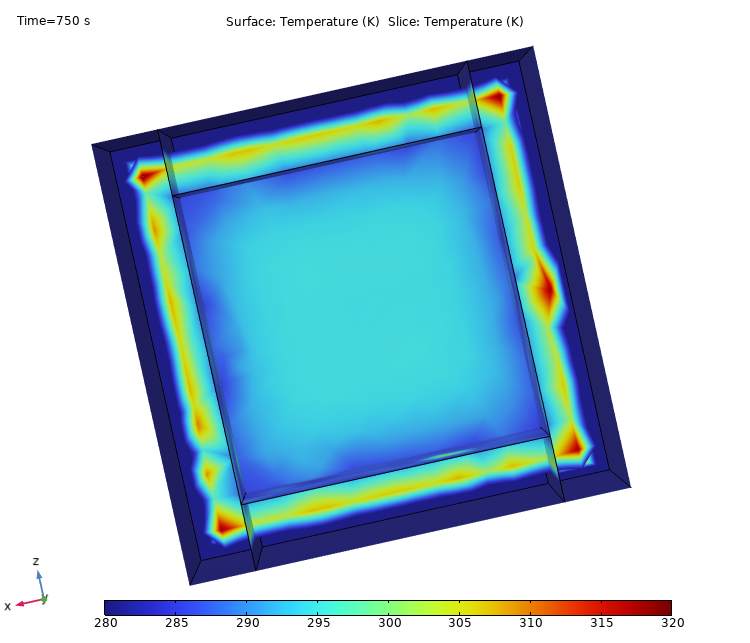
\includegraphics[width=0.3\textwidth]{cube/normal_750s.png}\hfill
\caption{Normal}
\label{cube-normal}
\end{figure}

\begin{figure}[H]
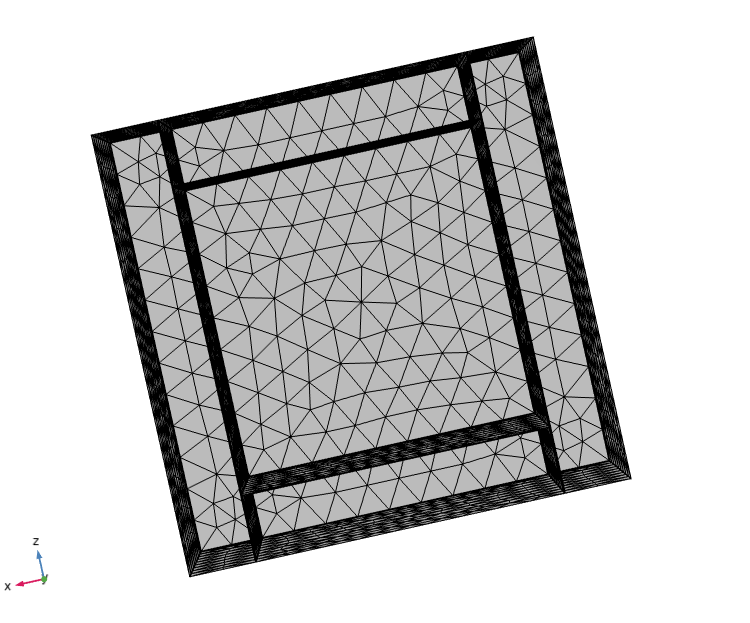
\includegraphics[width=0.3\textwidth]{cube/fine_mesh.png}\hfill
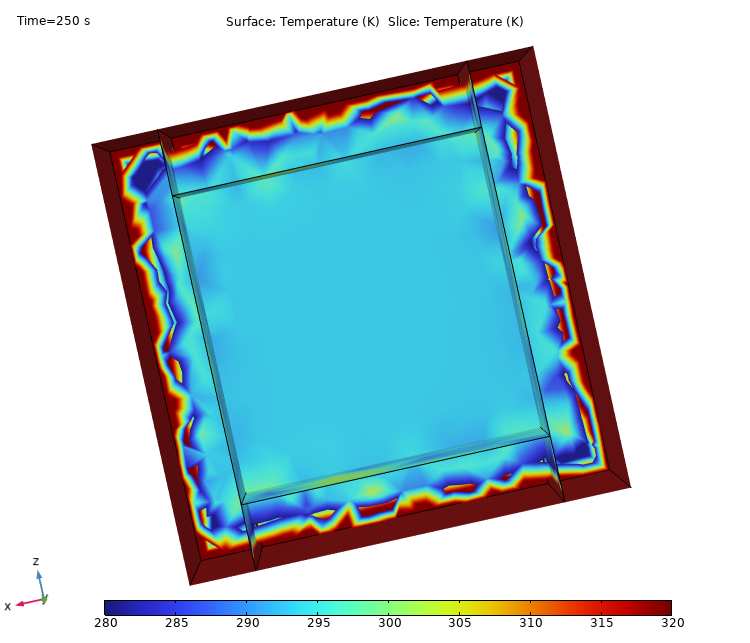
\includegraphics[width=0.3\textwidth]{cube/fine_250s.png}\hfill
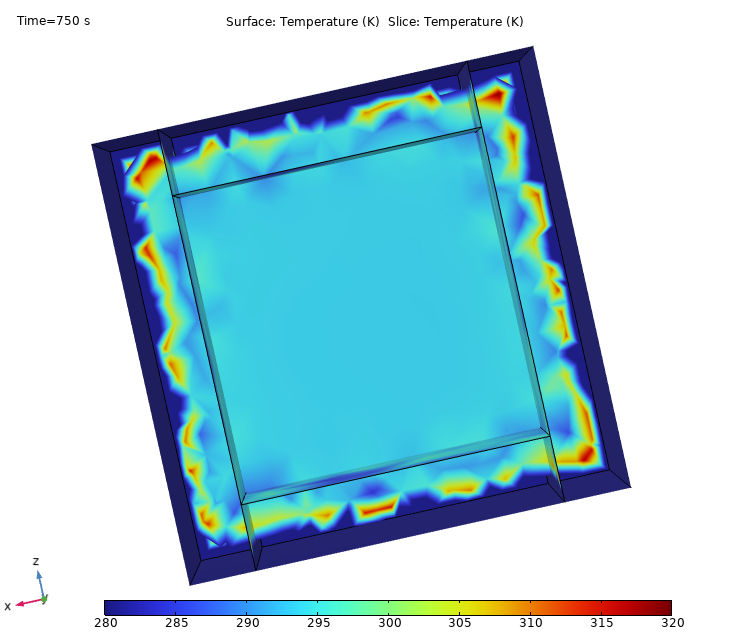
\includegraphics[width=0.3\textwidth]{cube/fine_750s.png}\hfill
\caption{Fine}
\label{cube-fine}
\end{figure}

\begin{figure}[H]
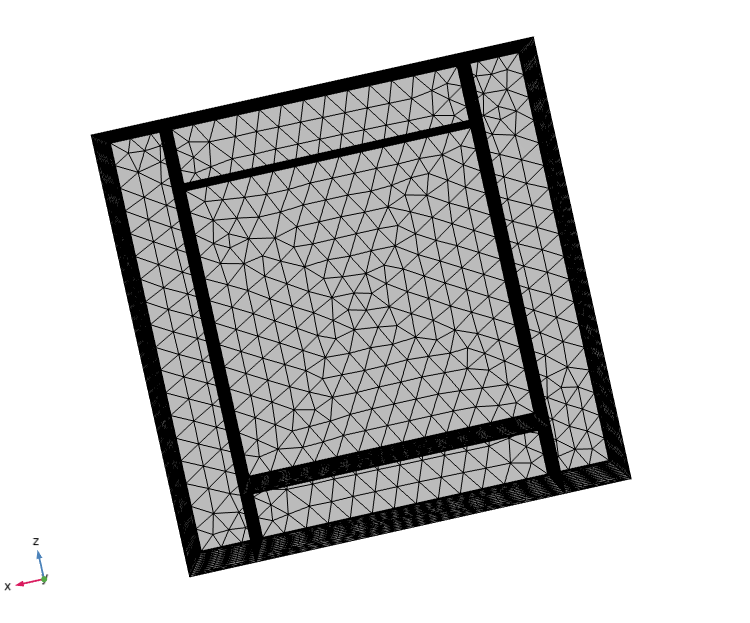
\includegraphics[width=0.3\textwidth]{cube/finer_mesh.png}\hfill
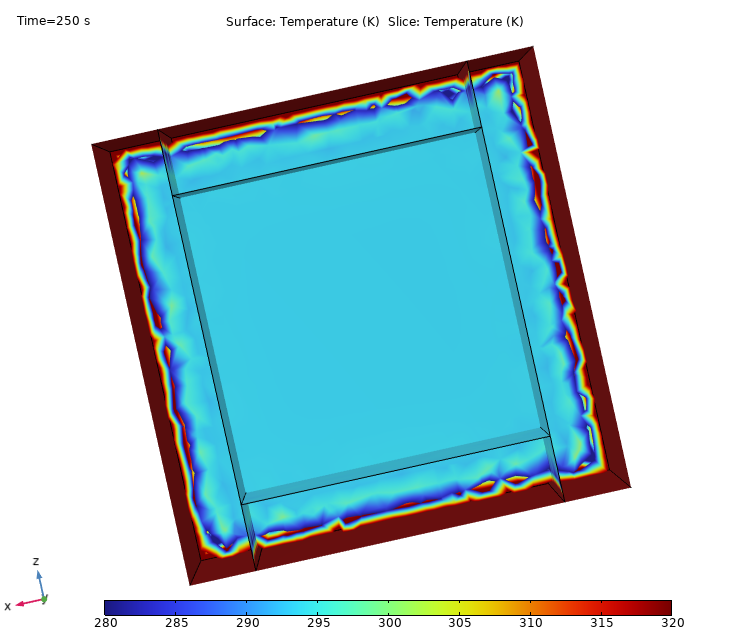
\includegraphics[width=0.3\textwidth]{cube/finer_250s.png}\hfill
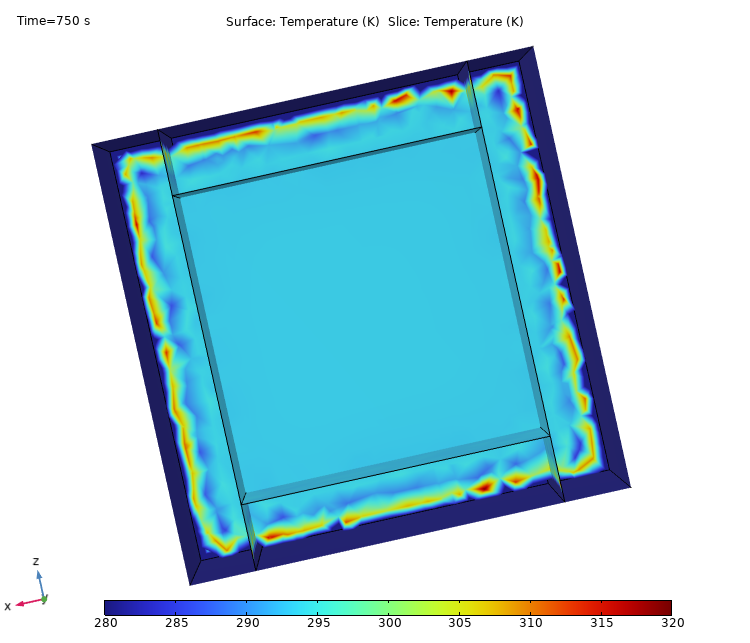
\includegraphics[width=0.3\textwidth]{cube/finer_750s.png}\hfill
\caption{Finer}
\label{cube-finer}
\end{figure}

\begin{figure}[H]
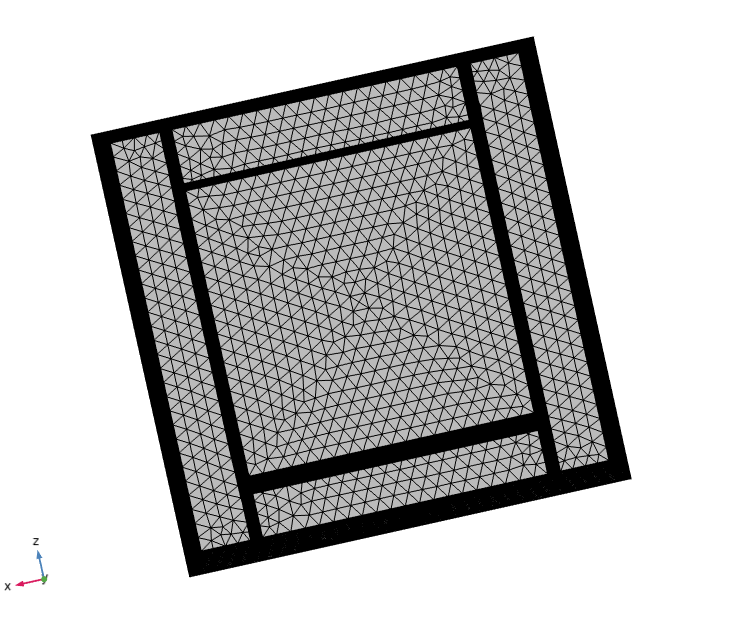
\includegraphics[width=0.3\textwidth]{cube/extra_fine_mesh.png}\hfill
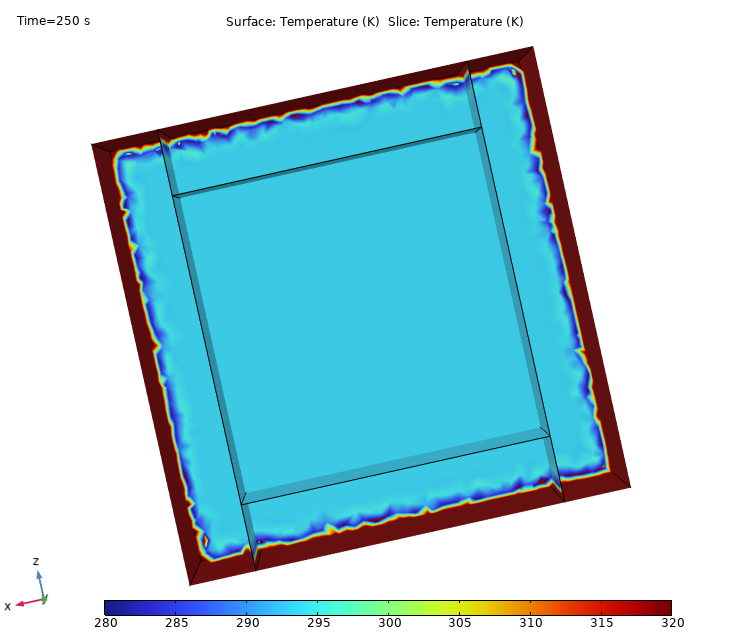
\includegraphics[width=0.3\textwidth]{cube/extra_fine_250s.png}\hfill
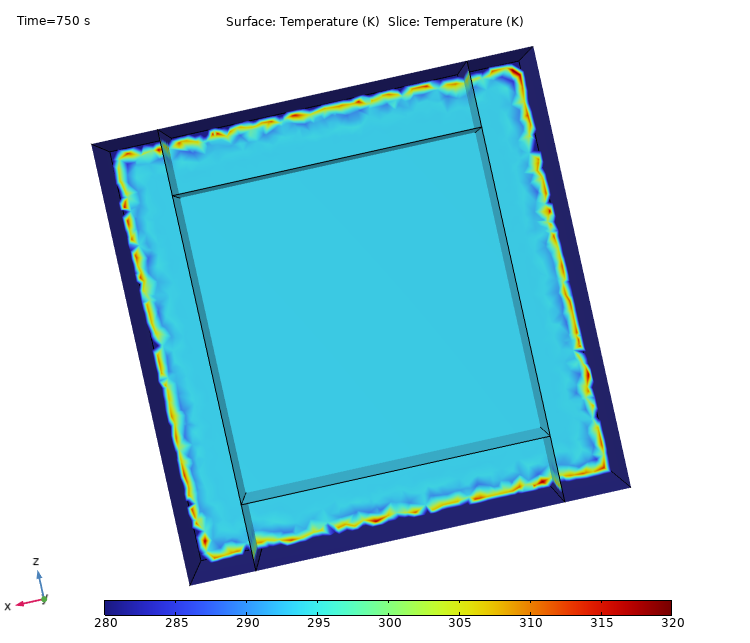
\includegraphics[width=0.3\textwidth]{cube/extra_fine_750s.png}\hfill
\caption{Extra fine}
\label{cube-extra-fine}
\end{figure}

Можно видеть, что у Normal и Fine сеток большая погрешность, тогда как начиная с Finer результат выглядит достаточно гладко. Время вычисления для Finer составило 20 секунд, для Extra fine - 80 секунд.\par
Была попытка запустить вычисления на сетке размером Extremely fine, но ожидаемое время было слишком большим и требовалось много памяти. В итоге было решено остановиться на Finer как достаточно точной при приемлемых затратах.

\newpage


\subsection{Построение модели помещения}

За основу было выбрано помещение, смоделированное в программе FreeCAD, экспортированное сначала в формат STL (но из-за особенности формата не подошло), затем в STEP (не удалось построить сетку разбиения из-за неточностей в геометрии помещения). В итоге было принято решение построить упрощенную модель сразу в COMSOL. Помещение размером $10 \times 6 \times 3 \text{ м}^3$ с окном, дверью и внутренней стеной с проходом. Материал стен - Concrete, дверь - Wood (pine), окно - Glass (quartz).

Начальная температура стен и воздуха внутри $20$ °C, внешняя температура задается синусоидой с периодом $24$ часа и амплитудой $4$ °C.
Временной промежуток $1$ день, шаг $5$ минут. Размер сетки Finer. При этом можно увидеть, что окно разбито на более мелкую сетку, чем все остальное (Рис. \ref{window}). Если отдельно сделать сетку для окна погрубее (Normal), то можно добиться снижения количества элементов разбиения на 22\% (в данном примере было $98659$, стало $76413$) без ухудшения качества.

\begin{figure}[H]
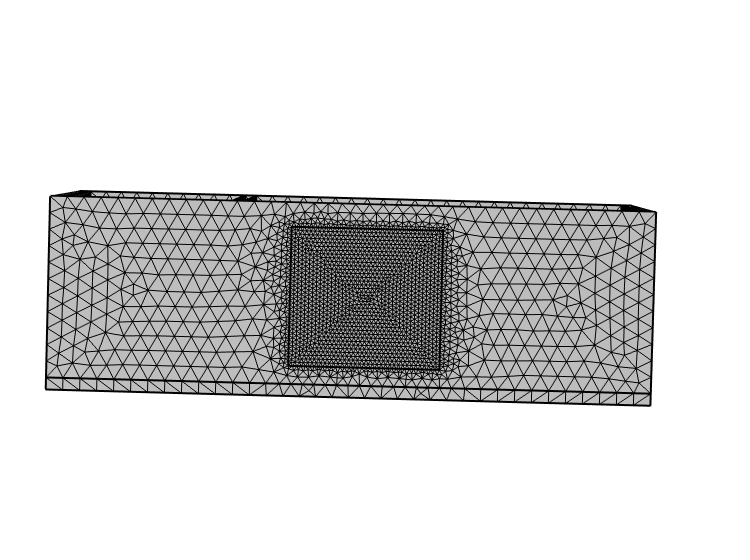
\includegraphics[width=0.5\textwidth]{smart_room/simple/window_finer.png}\hfill
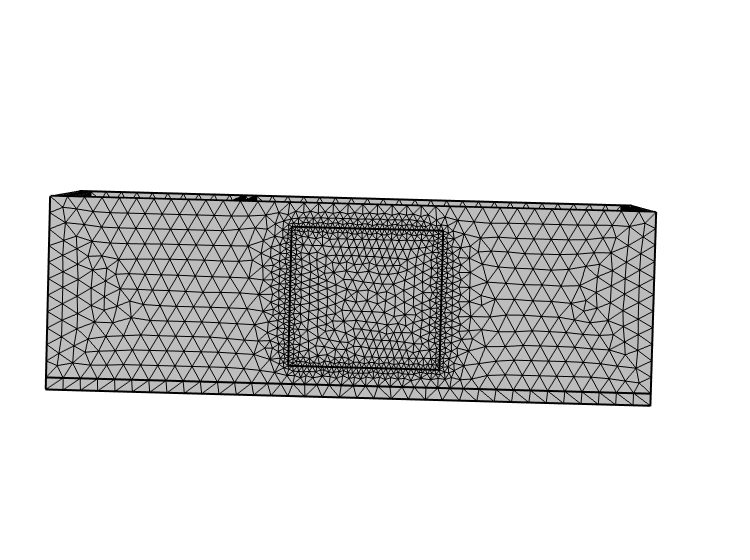
\includegraphics[width=0.5\textwidth]{smart_room/simple/window_normal.png}
\caption{Сетка разбиения окна}
\label{window}
\end{figure}


Полученные результаты можно увидеть на изображениях снизу. На них показана температура стен и температура воздуха в горизонтальном разрезе.

\begin{figure}[H]
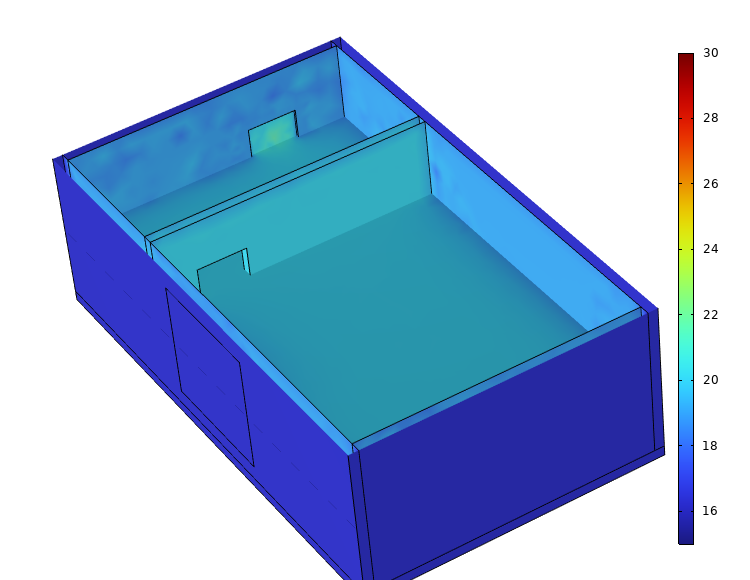
\includegraphics[width=0.5\textwidth]{smart_room/simple/finer_6h.png}\hfill
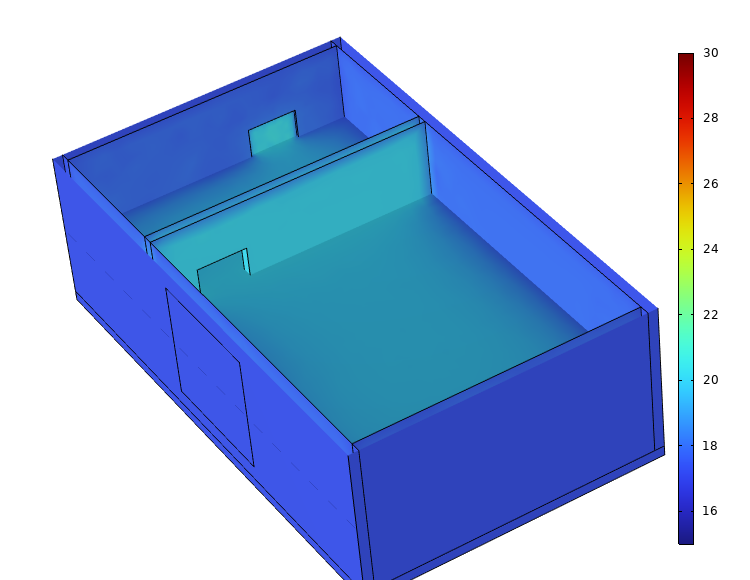
\includegraphics[width=0.5\textwidth]{smart_room/simple/finer_9h.png}
\caption{6 и 9 часов}
\end{figure}

\begin{figure}[H]
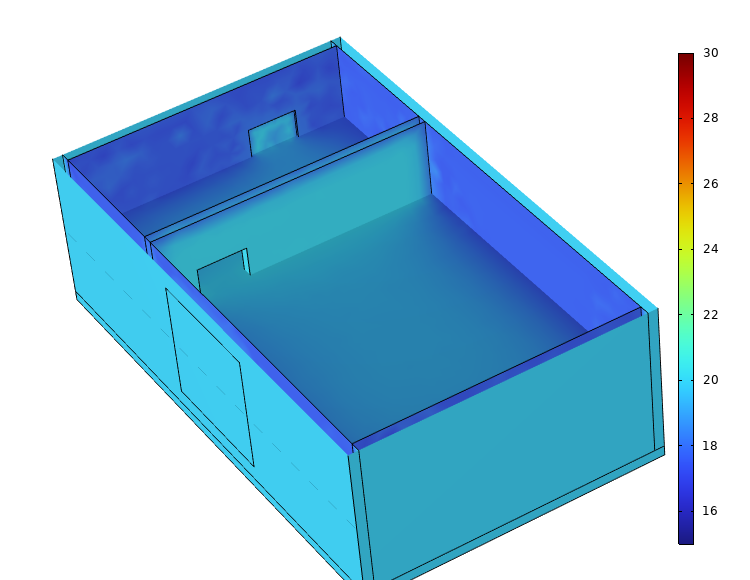
\includegraphics[width=0.5\textwidth]{smart_room/simple/finer_12h.png}\hfill
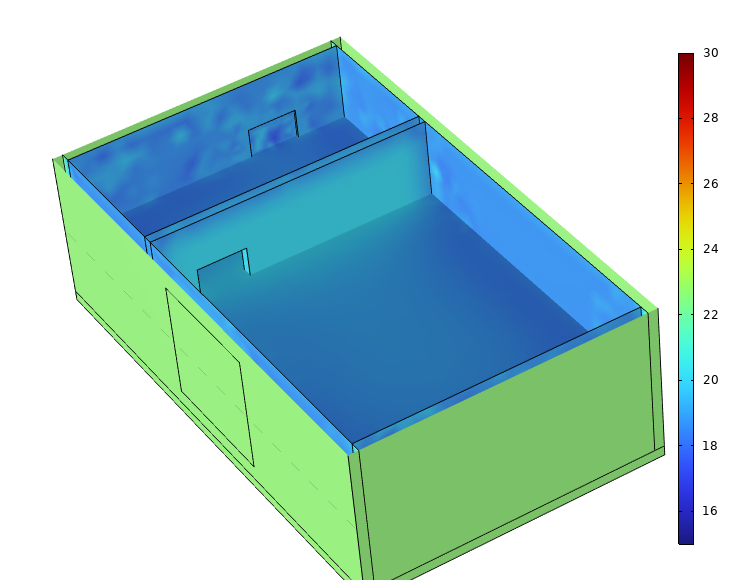
\includegraphics[width=0.5\textwidth]{smart_room/simple/finer_15h.png}
\caption{12 и 15 часов}
\end{figure}

\begin{figure}[H]
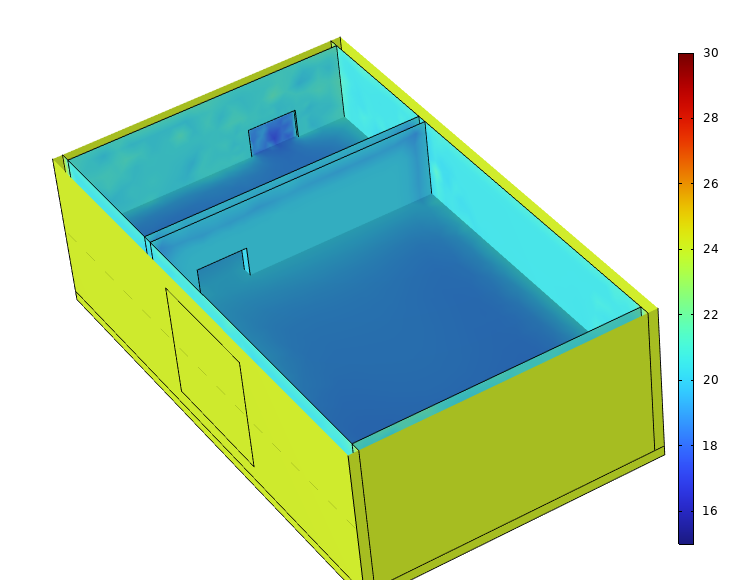
\includegraphics[width=0.5\textwidth]{smart_room/simple/finer_18h.png}\hfill
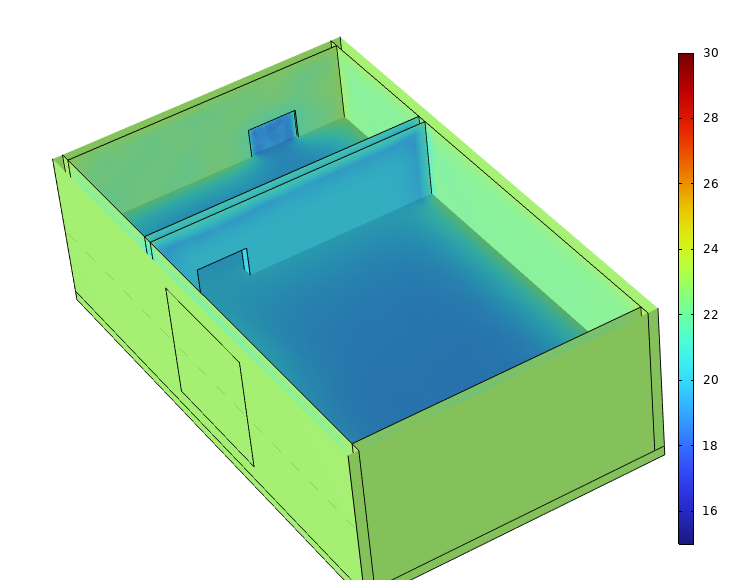
\includegraphics[width=0.5\textwidth]{smart_room/simple/finer_21h.png}
\caption{18 и 21 час}
\end{figure}
\newpage


\subsection{Моделирование с реальными данными температур}

Для моделирования погодных условий был использован датасет с температурами, использованный для прошлых исследований, за май-август 2020 года. В нем с шагом примерно 1 секунда записаны показания датчика, расположенного снаружи (Рис. \ref{real-temperature-plot}). Было решено промоделировать 4 дня с шагом в 5 минут. 

\begin{figure}[H]
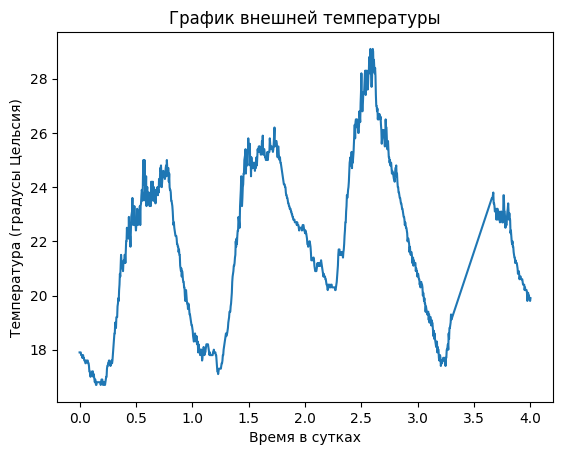
\includegraphics[width=\textwidth]{smart_room/real_temperature/temperature_plot.png}
\caption{График внешней температуры}
\label{real-temperature-plot}
\end{figure}

\newpage


\subsection{Добавление солнечной радиации}

Следующим шагом стало добавление солнечной радиации.
Все внешние стены комнаты и потолок, а также внутренние стены и пол, на которые могло светить солнце сквозь стекло, были подвержены тепловому излучению. Окно расположено стороной на юг.

В качестве источника радиации выбрано солнце, географическое расположение помещения - город Москва, дата 04.08.2020.
Полученные результаты ниже (Рис. \ref{fine-radiation}). На этих изображениях можно отметить нагрев части пола, на которую светит солнце через окно.

\begin{figure}[H]
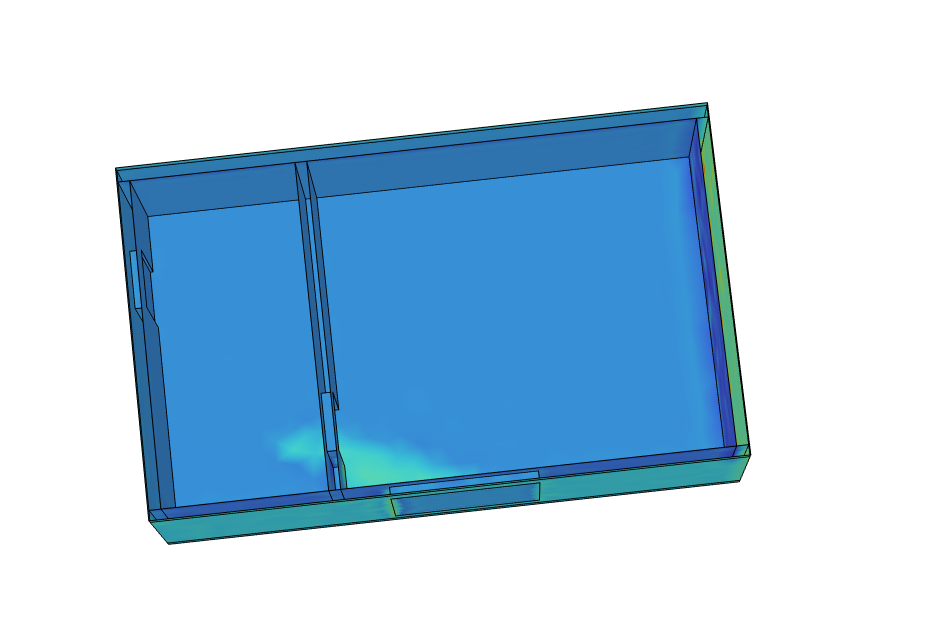
\includegraphics[width=0.5\textwidth]{smart_room/solar_radiation/fine_1.png}\hfill
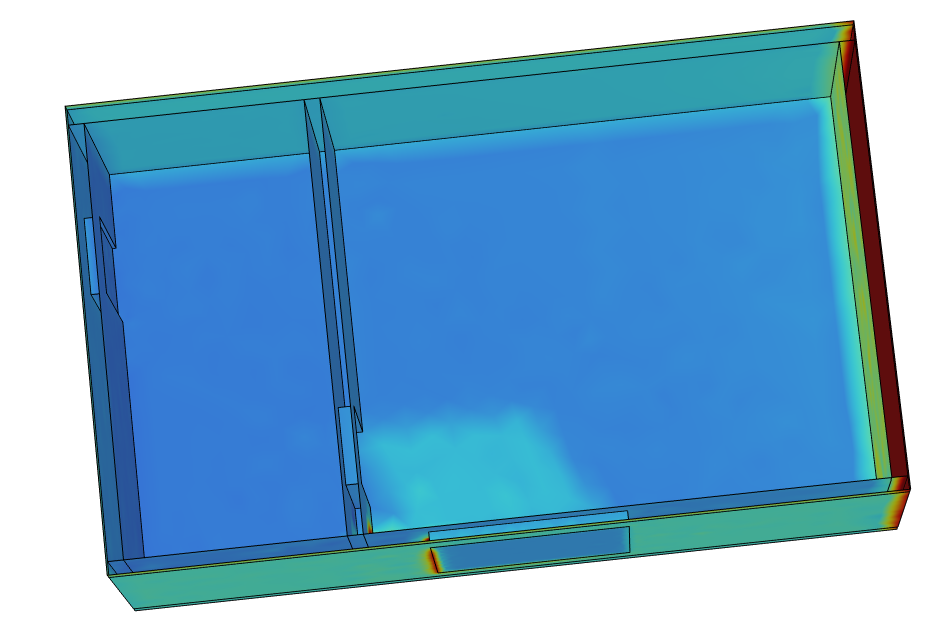
\includegraphics[width=0.5\textwidth]{smart_room/solar_radiation/fine_2.png}\hfill
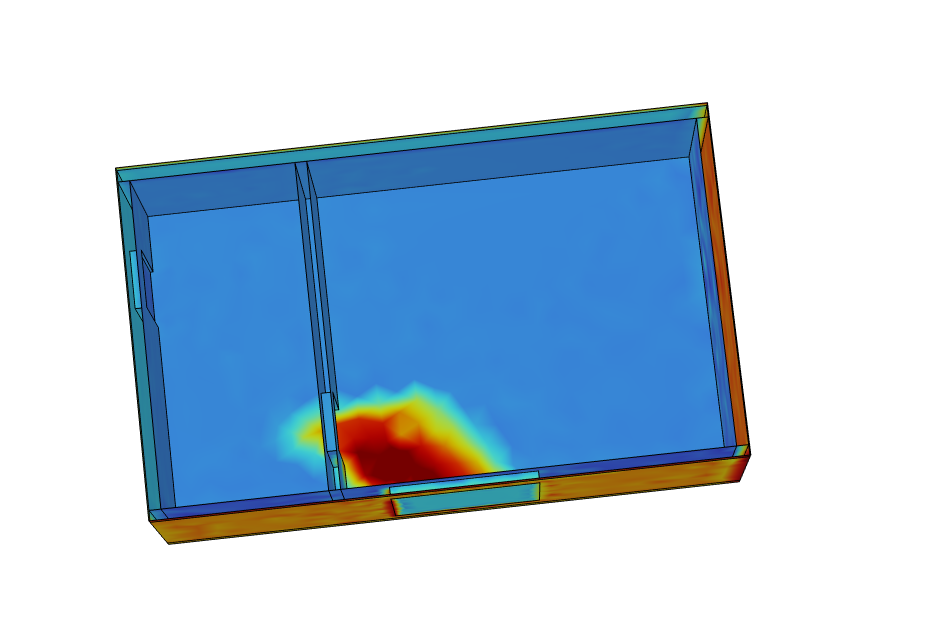
\includegraphics[width=0.5\textwidth]{smart_room/solar_radiation/fine_3.png}\hfill
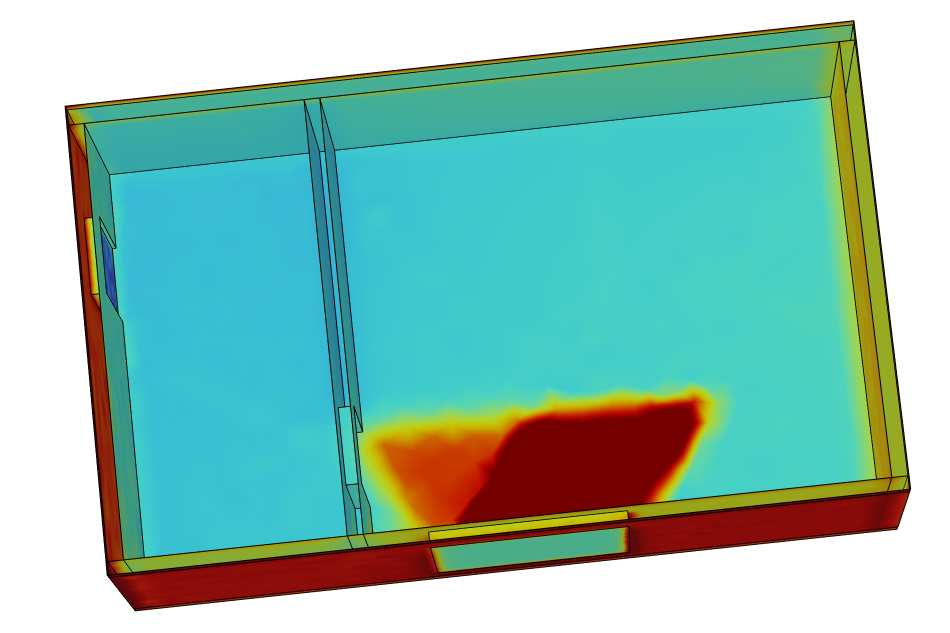
\includegraphics[width=0.5\textwidth]{smart_room/solar_radiation/fine_4.png}\hfill
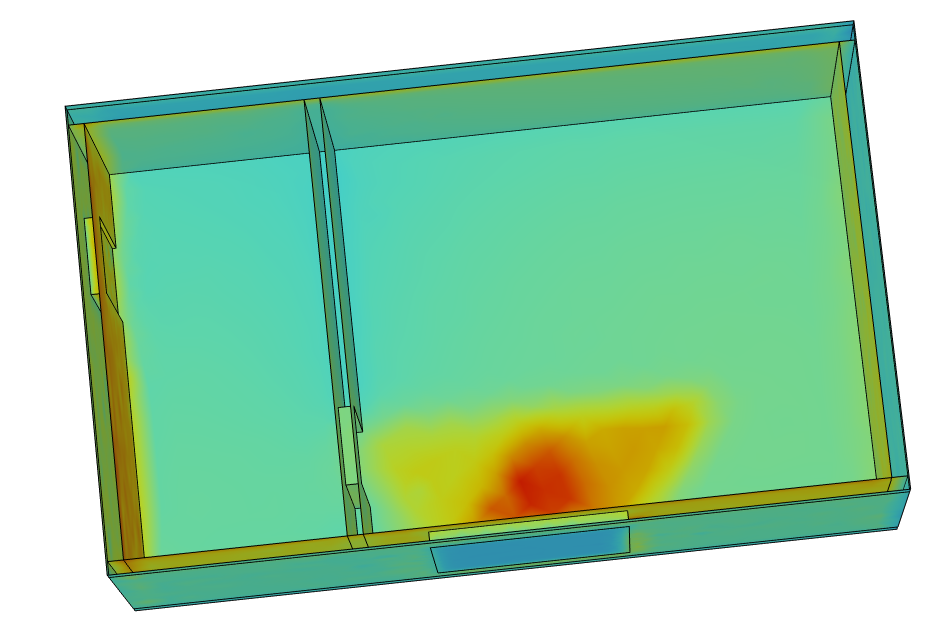
\includegraphics[width=0.5\textwidth]{smart_room/solar_radiation/fine_5.png}\hfill
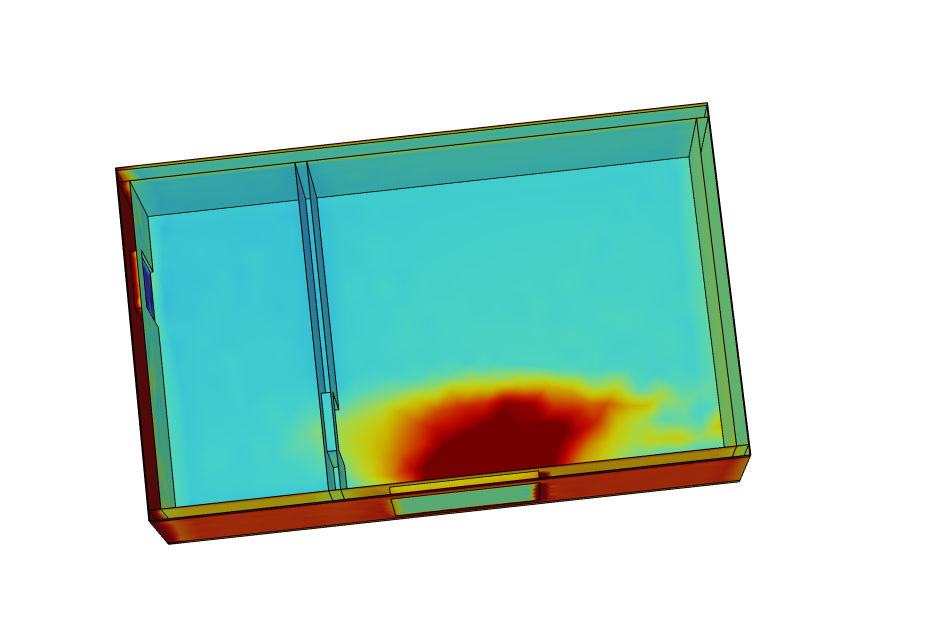
\includegraphics[width=0.5\textwidth]{smart_room/solar_radiation/fine_6.png}\hfill
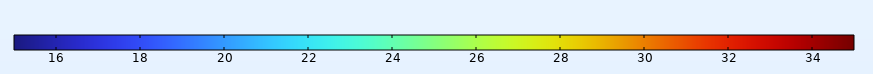
\includegraphics[width=\textwidth]{smart_room/solar_radiation/fine_color_legend.png}\hfill
\caption{}
\label{fine-radiation}
\end{figure}













































\graphicspath{{./images/algo}}
\section{Аналитическая часть}

\subsection{Экспортирование результата в таблицу}

Для нахождения оптимального расположения датчика, будем перебирать интересующие точки, и температуру в них запишем в таблицу для дальнейшего сравнения. Самым простым вариантом будет рассмотреть сетку из точек $9 \times 9 \times 9$ (Рис. \ref{9x9x9}).

\begin{figure}[H]
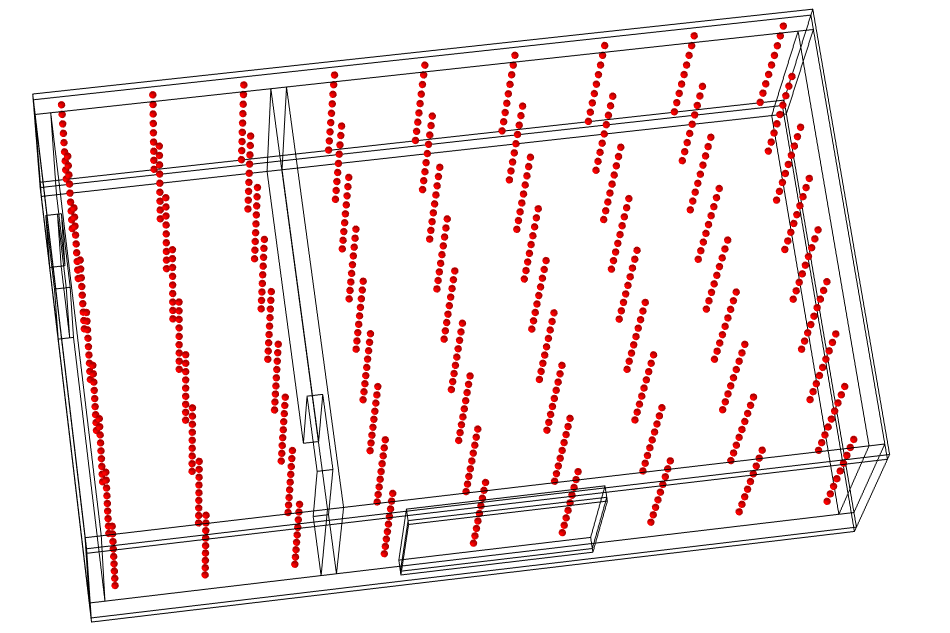
\includegraphics[width=\textwidth]{comsol/interesting_points_9x9x9.png}
\caption{}
\label{9x9x9}
\end{figure}

Однако можно заметить, что большинство точек находятся не у стены, а значит и установить датчик в них будет проблематично. Поэтому более оптимальным вариантом будет рассмотреть сетку вдоль каждой из стен, пола и потолка (Рис. \ref{interesting_points}). Точки будем распологать на некотором расстоянии от стены ($15$ см), так как температура воздуха может достаточно сильно отличаться от температуры стены.

\begin{figure}[H]
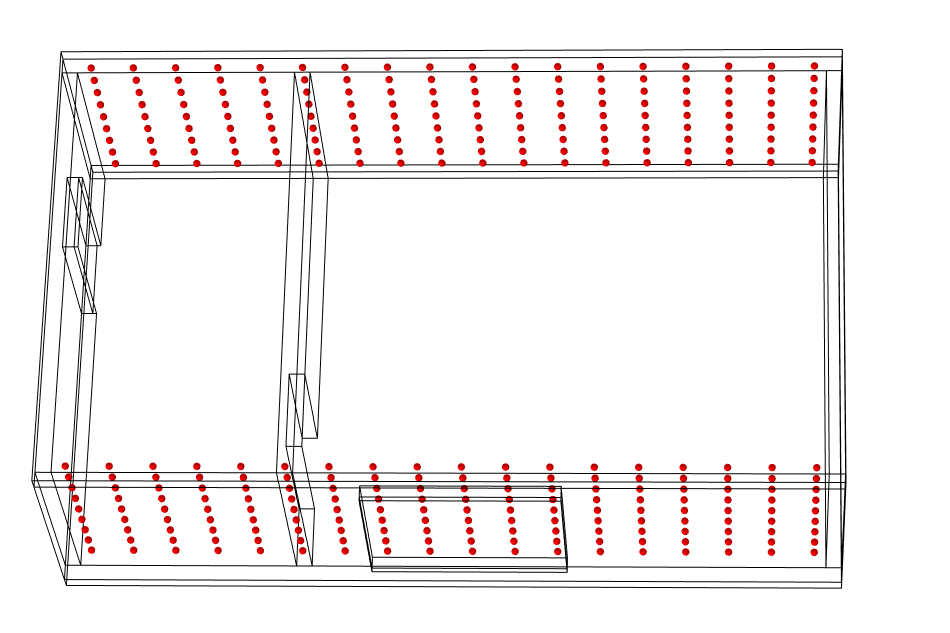
\includegraphics[width=0.5\textwidth]{comsol/interesting_points_X.png}
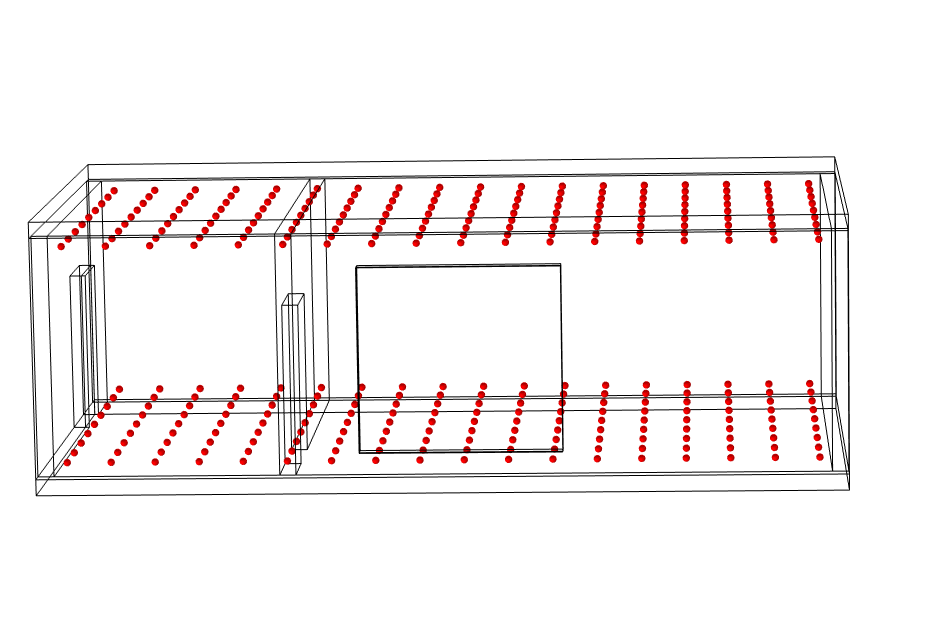
\includegraphics[width=0.5\textwidth]{comsol/interesting_points_Z.png}
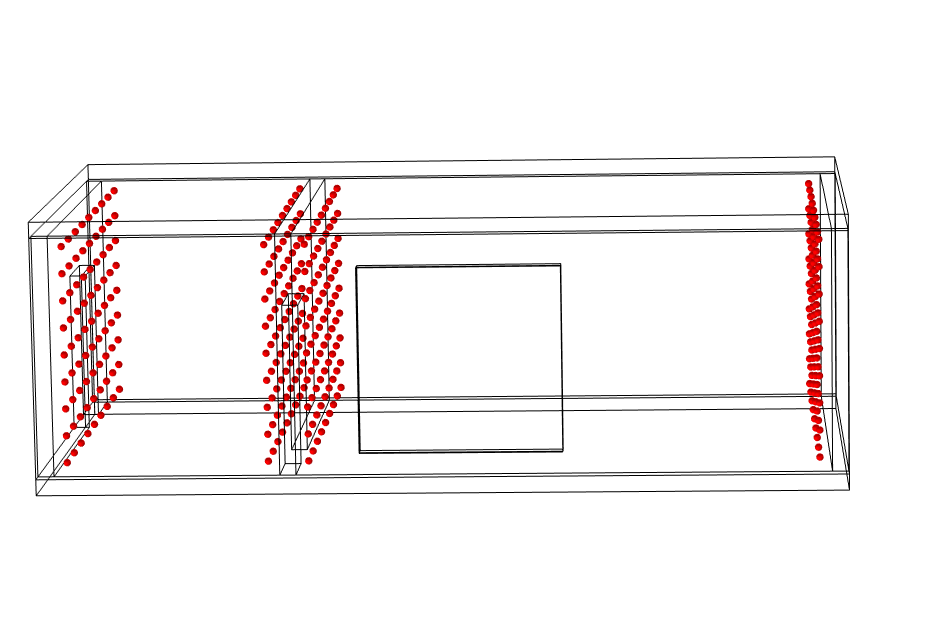
\includegraphics[width=\textwidth]{comsol/interesting_points_Y.png}
\caption{}
\label{interesting_points}
\end{figure}

Полученная таблица температур выглядит так:

\begin{table}[H]
\centering
\begin{tabular}{c|c|c|c|c|c}
\textbf{Time (s)} & \textbf{Point 1} & \textbf{Point 2} & ... & \textbf{Point N} & \textbf{Ambient} \\ \hline
0                 & 20.0             & 19.4             &     & 20.8              & 17.9             \\
300               & 19.9             & 19.4             &     & 20.7              & 17.9             \\
600               & 19.9             & 19.4             &     & 20.6              & 17.9             \\
...               &                  &                  &     &                   &                  \\
345600            & 21.2             & 21.5             &     & 20.8              & 19.9            
\end{tabular}
\end{table}

\newpage


\subsection{Критерий оптимальности точки}
\label{algo-2}

Теперь надо определить критерий оптимальности точки. Между внутренней температурой помещения и внешней температурой есть явная линейная зависимость \cite{pashchenko-rassadin}. Однако, для нахождения наиболее точной регрессии, надо определить временной сдвиг температур. Из физической сущности процесса тепломассообмена следует, что нагрев и охлаждение помещения под воздействием наружной температуры происходит не мгновенно, а с некоторым временным сдвигом. Например, на графике (Рис. \ref{indent1}) изображено изменение внешней температуры (синяя кривая) и температура в одной из внутренних точек (оранжевая кривая). Можно видеть, что точки перелома у синей кривой встречаются раньше, чем у оранжевой.

\begin{figure}[H]
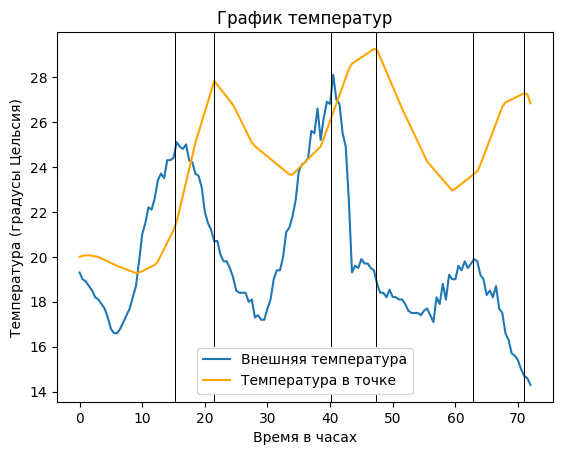
\includegraphics[width=\textwidth]{graphics/indent.png}
\caption{}
\label{indent1}
\end{figure}

\newpage

Величину этого сдвига будем определять, сдвигая последовательно массив значений наружной температуры относительно массива внутренней температуры на шаг $t$ и вычисляя значение линейной корреляции Пирсона \cite{pearson} между полученными рядами. В нашем случае шаг $t$ равен шагу в модели и составляет $5$ минут. На полученном графике (Рис. \ref{indent2}) видно, что после сдвига точки экстремума гораздо лучше накладываются друг на друга, что в свою очередь улучшает точность линейной регрессии. Сдвиг при этом для каждой точки может быть разный.

\begin{figure}[H]
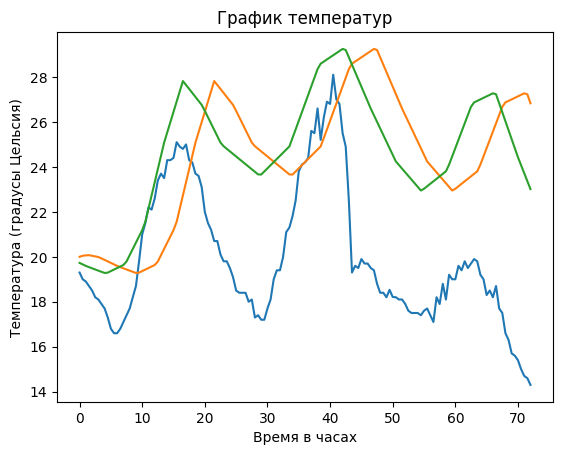
\includegraphics[width=\textwidth]{graphics/indent_2.png}
\caption{}
\label{indent2}
\end{figure}

\newpage 


\subsection{Описание алгоритма}

Теперь, когда определили временной сдвиг, можем строить линейную регрессию. Для этого у нас есть 2 датасета: тренировочный, в котором записаны посчитанные температуры за 4 дня с 04.08.2020 по 07.08.2020, и тестовый, в котором температуры за 3 дня с 09.08.2020 по 11.08.2020. Мы перебираем все возможные столбцы температур из тренировочной таблицы, для каждой находим свой сдвиг, при котором коэффициент линейной корреляции Пирсона со столбцом внешних температур максимален. Затем считаем коэффициенты линейной регрессии сдвинутого столбца. Далее, используя полученные коэффициенты и сдвиг, аппроксимируем температуру воздуха снаружи из тестового датасета. Для полученной аппроксимации считаем коэффициент детерминации $R^2$. Точка с наибольшим коэффициентом считается оптимальной.

На графике ниже (Рис. \ref{result}) показан результат работы алгоритма. 

\begin{figure}[H]
\centering
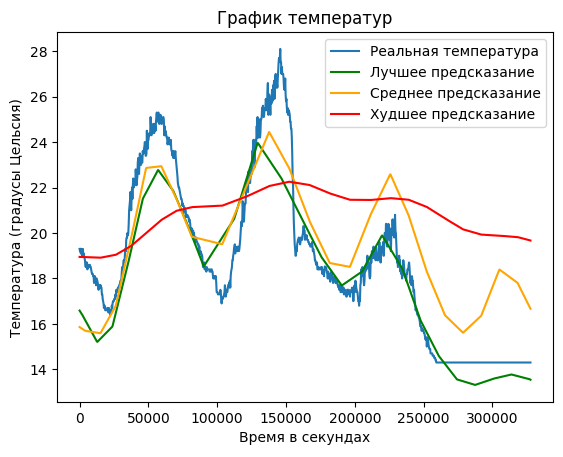
\includegraphics[width=0.9\textwidth]{graphics/result.png}
\caption{}
\label{result}
\end{figure}

Можно видеть, что в точках локальных минимумов и максимумов разница предсказаний доходит до $2$-х градусов между лучшим и средним. Худшее же предсказание показывает наименьшее колебание температур. Точка с худшим предсказанием находится в самом центре комнаты (Рис. \ref{interesting-points-result}). Это логичный результат, так как все остальные точки находятся рядом со стенами, которые напрямую взаимодействуют с окружающей средой, и поэтому температура в них также сильнее зависит от внешней температуры. Лучшее расположение датчика оказывается рядом со стеклом, что тоже логично, так как на стены светит солнце и излишне нагревает их. Окно в свою очередь не подвержено солнечной радиации, поэтому и температура будет зависеть в основном от внешней. Для остальных точек сложнее делать выводы, так как точки над окном находятся на юге, а значит и греются больше всего. Тем не менее, предсказания в них являются лучшими после точки у окна.

Также нужно учитывать саму модель. Данное помещение смоделировано как отдельное здание, а не как одна комната в большом доме. То есть все стены и потолок взаимодействуют со внешней средой, на них светит солнце. Для комнаты было бы так, что температура внутренних стен была бы более стабильной, а значит и результаты предсказаний были бы другими.


\begin{figure}[H]
\centering
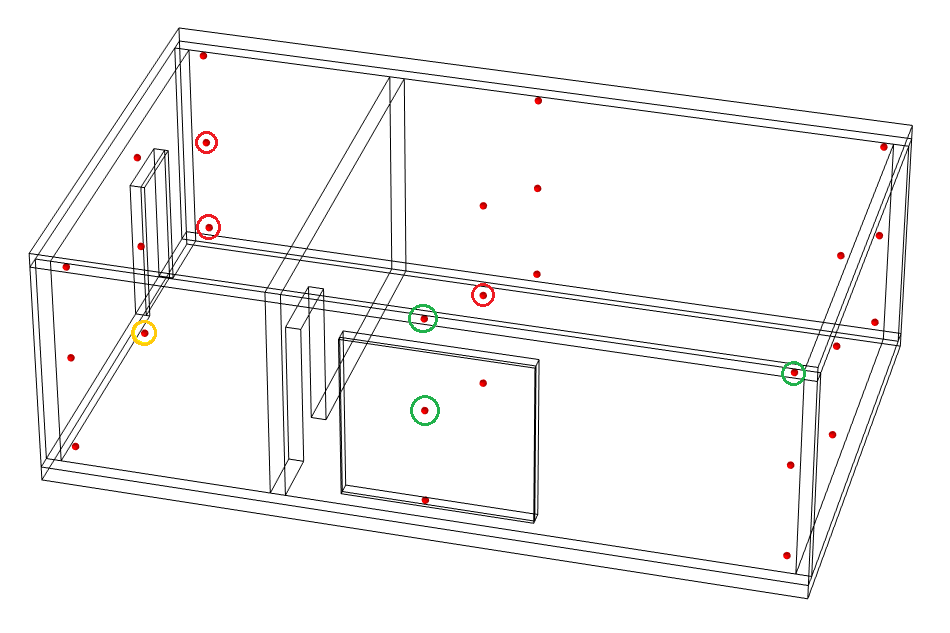
\includegraphics[width=0.9\textwidth]{interesting_points_result.png}
\caption{}
\label{interesting-points-result}
\end{figure}










































\specialsection{Заключение}

Заключение должно подводить итоги работы и содержать информацию о полученных в рамках работы результатах.

\newpage
% Аргумент {1} ниже включает переопределенный стиль с выравниванием слева
\begin{thebibliography}{1}
\bibitem{comsol} COMSOL Multiphysics®. URL: \url{https://www.comsol.ru}.
\end{thebibliography}

\end{document}